% ============================================================================
% CHAPTER 2: SYSTEM ANALYSIS
% ============================================================================

\chapter{SYSTEM ANALYSIS}

\section{EXISTING SYSTEM}

This section provides a detailed analysis of the base paper by Khaleghi et al. \cite{khaleghi2025interpretable}, published in MethodsX (2025), which serves as the primary reference point for understanding the current state of the art and identifying opportunities for improvement in EEG-based depression detection.

\subsection{Base Paper Overview}

The base paper presents an interpretable deep learning approach for depression detection using EEG signals, representing a recent contribution to the growing literature on automated psychiatric diagnosis. The authors utilize the Kaggle Depression-Rest EEG Dataset containing recordings from 232 patients and employ a relatively straightforward machine learning pipeline. Their approach begins with 31 pre-extracted features spanning six brain regions, applies Principal Component Analysis (PCA) for dimensionality reduction to 21 components, and feeds the resulting feature vectors into a two-layer convolutional neural network for classification. The paper incorporates SHAP (SHapley Additive exPlanations) for model interpretability and reports an impressive 98\% classification accuracy using 5-fold stratified cross-validation. Table \ref{tab:base_paper_summary} summarizes the key characteristics of this approach.

\begin{table}[H]
    \centering
    \small
    \caption{Summary of Base Paper Approach (Khaleghi et al., 2025)}
    \label{tab:base_paper_summary}
    \begin{tabularx}{\textwidth}{|L{3.5cm}|X|}
        \hline
        \textbf{Aspect} & \textbf{Description} \\
        \hline
        Dataset & Kaggle Depression-Rest EEG Dataset (232 patients) \\
        \hline
        Features & 31 pre-extracted features across 6 brain regions \\
        \hline
        Dimensionality Reduction & PCA (21 components) + t-SNE for visualization \\
        \hline
        Model Architecture & 2-layer CNN (64 and 128 filters) \\
        \hline
        Validation & 5-fold stratified cross-validation \\
        \hline
        Interpretability & SHAP (SHapley Additive exPlanations) \\
        \hline
        Reported Accuracy & 98\% \\
        \hline
    \end{tabularx}
\end{table}

\subsection{Base Paper Architecture}

The base paper employs a relatively simple convolutional neural network architecture consisting of two convolutional layers followed by fully connected layers for classification. The network receives the 21 PCA-reduced features as input, which are first reshaped into a single-channel one-dimensional signal format suitable for convolutional processing. The first convolutional layer applies 64 filters with kernel size 3, followed by max pooling that reduces the spatial dimension by half. The second convolutional layer increases the representational capacity with 128 filters, again followed by max pooling. After flattening the resulting feature maps, a dense layer with 64 units and ReLU activation provides the final feature transformation before the output layer produces class probabilities through softmax activation. Table \ref{tab:base_cnn_arch} details the complete architecture specifications, revealing a total parameter count of approximately 50,000---a relatively modest capacity for the complexity of the classification task.

\begin{table}[H]
    \centering
    \small
    \caption{Base Paper CNN Architecture Specifications}
    \label{tab:base_cnn_arch}
    \begin{tabularx}{\textwidth}{|l|l|l|X|}
        \hline
        \textbf{Layer} & \textbf{Type} & \textbf{Configuration} & \textbf{Output Shape} \\
        \hline
        Input & --- & 21 PCA features & (batch, 21) \\
        \hline
        Reshape & Reshape & --- & (batch, 1, 21) \\
        \hline
        Conv1 & Conv1D & 64 filters, kernel=3 & (batch, 64, 19) \\
        \hline
        Pool1 & MaxPool1D & pool\_size=2 & (batch, 64, 9) \\
        \hline
        Conv2 & Conv1D & 128 filters, kernel=3 & (batch, 128, 7) \\
        \hline
        Pool2 & MaxPool1D & pool\_size=2 & (batch, 128, 3) \\
        \hline
        Flatten & Flatten & --- & (batch, 384) \\
        \hline
        Dense1 & Dense & 64 units, ReLU & (batch, 64) \\
        \hline
        Output & Dense & 2 units, Softmax & (batch, 2) \\
        \hline
    \end{tabularx}
\end{table}

\begin{figure}[H]
    \centering
    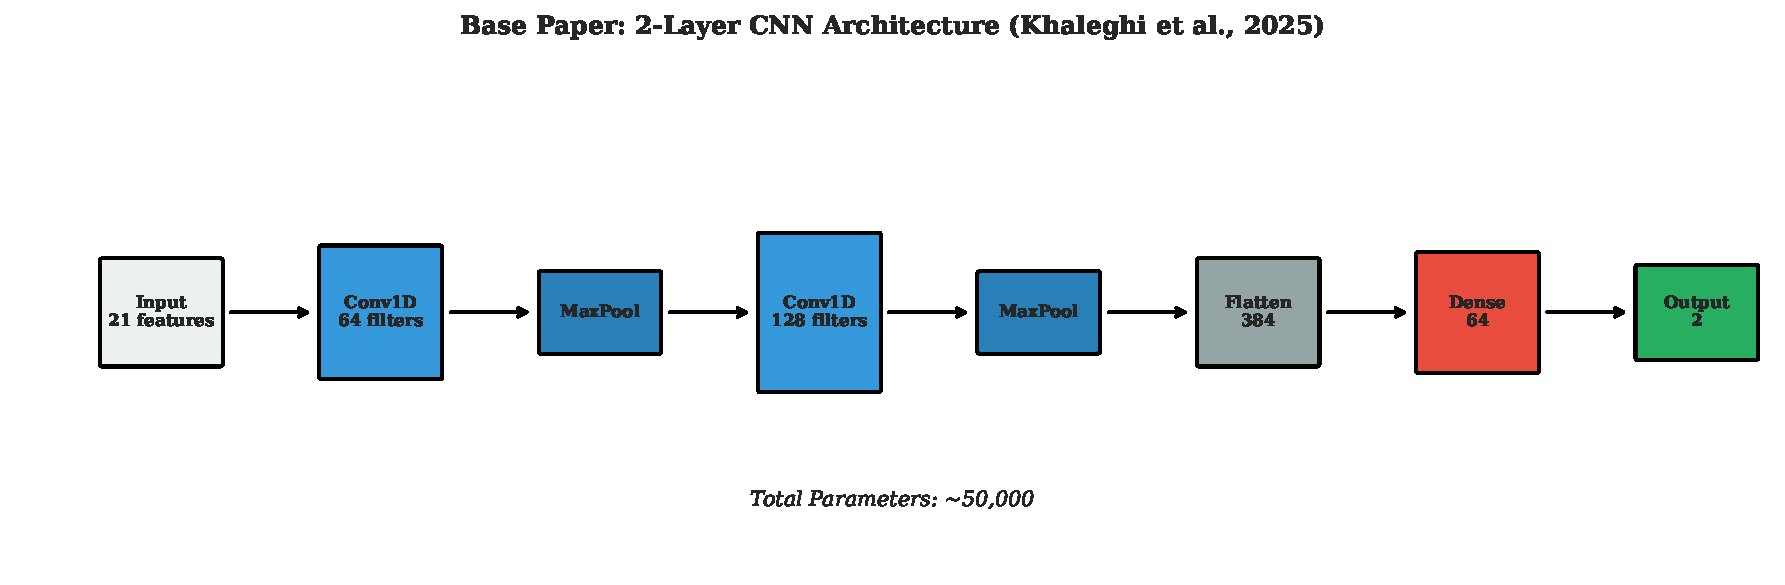
\includegraphics[width=0.9\textwidth]{figures/ch2/fig2_1_base_cnn.pdf}
    \caption{Base paper 2-layer CNN architecture for depression classification.}
    \label{fig:base_cnn_arch}
\end{figure}

\subsection{Base Paper Feature Extraction}

The base paper utilizes 31 pre-extracted features from the Kaggle dataset, organized into six categories spanning different aspects of EEG signal characterization. Spectral features capture band power in the standard frequency ranges including delta (1-4 Hz), theta (4-8 Hz), alpha (8-13 Hz), beta (13-30 Hz), and gamma (30-45 Hz) bands, computed using Fast Fourier Transform methods. Ratio features represent cross-band relationships such as delta-to-alpha and theta-to-beta power ratios, which have been associated with various cognitive and emotional states. Asymmetry features quantify hemispheric differences in power, particularly relevant given the established literature on frontal alpha asymmetry in depression. Entropy features based on wavelet decomposition provide measures of signal complexity and irregularity. Statistical features including mean, variance, and skewness capture basic distributional properties of the signals. Finally, regional features aggregate information across anatomically meaningful electrode groups including frontal, temporal, parietal, and occipital regions. Table \ref{tab:base_features} summarizes these feature categories.

\begin{table}[H]
    \centering
    \small
    \caption{Base Paper Feature Categories}
    \label{tab:base_features}
    \begin{tabularx}{\textwidth}{|L{2.5cm}|L{3.5cm}|X|}
        \hline
        \textbf{Category} & \textbf{Features} & \textbf{Description} \\
        \hline
        Spectral & Delta, Theta, Alpha, Beta, Gamma power & FFT-based band power in standard frequency bands \\
        \hline
        Ratio Features & Delta/Alpha, Theta/Beta ratios & Cross-band power ratios \\
        \hline
        Asymmetry & Left-Right differences & Hemispheric power differences \\
        \hline
        Entropy & Wavelet entropy & Signal complexity measure \\
        \hline
        Statistical & Mean, variance, skewness & Basic statistical moments \\
        \hline
        Regional & Frontal, temporal, parietal, occipital & Region-specific aggregations \\
        \hline
    \end{tabularx}
\end{table}

\begin{figure}[H]
    \centering
    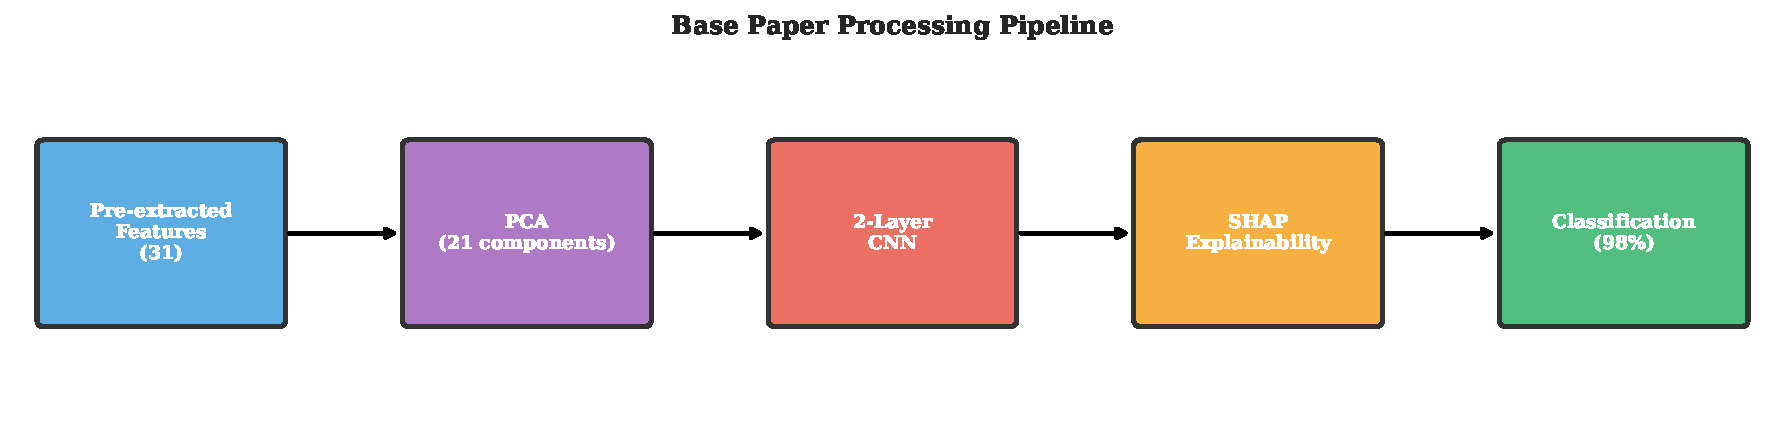
\includegraphics[width=0.9\textwidth]{figures/ch2/fig2_2_base_pipeline.pdf}
    \caption{Base paper processing pipeline showing the flow from pre-extracted features to classification.}
    \label{fig:base_pipeline}
\end{figure}

\subsection{Critical Analysis of Base Paper Limitations}

While the base paper reports impressive results, our thorough analysis reveals several significant methodological limitations that fundamentally undermine the clinical utility and scientific validity of the reported findings.

\subsubsection{Limitation 1: Data Leakage in Cross-Validation}

The most critical limitation is the use of standard 5-fold cross-validation without subject-wise splitting, which introduces severe data leakage that invalidates the reported performance metrics. With 232 patients contributing multiple samples each, random splitting inevitably causes epochs from the same subject to appear in both training and test sets. This allows the model to achieve artificially high accuracy by learning subject-specific patterns rather than depression-related patterns.

Several pieces of evidence strongly suggest the presence of data leakage in the reported results. The claimed 98\% accuracy is suspiciously high for a complex psychiatric classification task, as even expert clinicians do not achieve such reliability in depression diagnosis. Furthermore, the model confidence scores reported in the paper range from 0.41 to 0.59 despite the 98\% accuracy, revealing poor calibration that would not be expected from a model genuinely learning disease-relevant patterns. Most tellingly, the paper reports only sample-level accuracy metrics without any subject-level evaluation, obscuring whether the model generalizes to new individuals or merely memorizes subject-specific characteristics.

\subsubsection{Limitation 2: Pre-Extracted Features}

The reliance on pre-extracted features from the Kaggle dataset severely limits methodological control and constrains the potential for innovation. Working with pre-extracted features means researchers cannot apply custom wavelet families that might be optimized for depression-specific frequency patterns. The fixed feature set prevents generation of time-frequency representations such as scalograms that would enable more sophisticated deep learning architectures like Transformers. Experimentation with different preprocessing pipelines---including alternative filtering parameters, artifact rejection strategies, or epoch segmentation approaches---becomes impossible when starting from pre-extracted features. Additionally, the aggregated regional features preclude extraction of channel-wise information necessary for graph-based spatial modeling that could capture electrode relationships. These constraints fundamentally limit the scientific exploration possible within this framework.

\subsubsection{Limitation 3: Simple Architecture}

The 2-layer CNN architecture, while computationally efficient, has severely limited representational capacity that constrains its ability to learn the complex patterns associated with depression. Convolutional layers with small kernels can only capture local patterns and cannot model long-range temporal dependencies that are crucial for EEG rhythms spanning multiple cycles. The architecture includes no mechanism for explicitly modeling spatial relationships between electrodes, treating the input as a simple one-dimensional sequence rather than a spatially organized array of sensors. The limited receptive field prevents the network from recognizing complex patterns that span the full input, and the approximately 50,000 parameters provide insufficient capacity for learning the nuanced feature transformations needed to distinguish depression from healthy brain states.

\subsubsection{Limitation 4: Limited Explainability}

While the base paper incorporates SHAP for model interpretability, this provides only a single, limited view of model decision-making that falls short of clinical requirements for understanding automated diagnostic systems. SHAP analysis reveals which input features contribute to predictions but cannot validate whether the model has learned specific clinical concepts that clinicians recognize and trust. There is no layer-wise understanding of how information flows through the network, making it difficult to understand what transformations the model applies to raw features. Most critically, SHAP cannot directly test hypotheses about whether the model uses established depression biomarkers such as frontal alpha asymmetry or elevated theta power, leaving uncertainty about the clinical validity of the learned representations.

\begin{figure}[H]
    \centering
    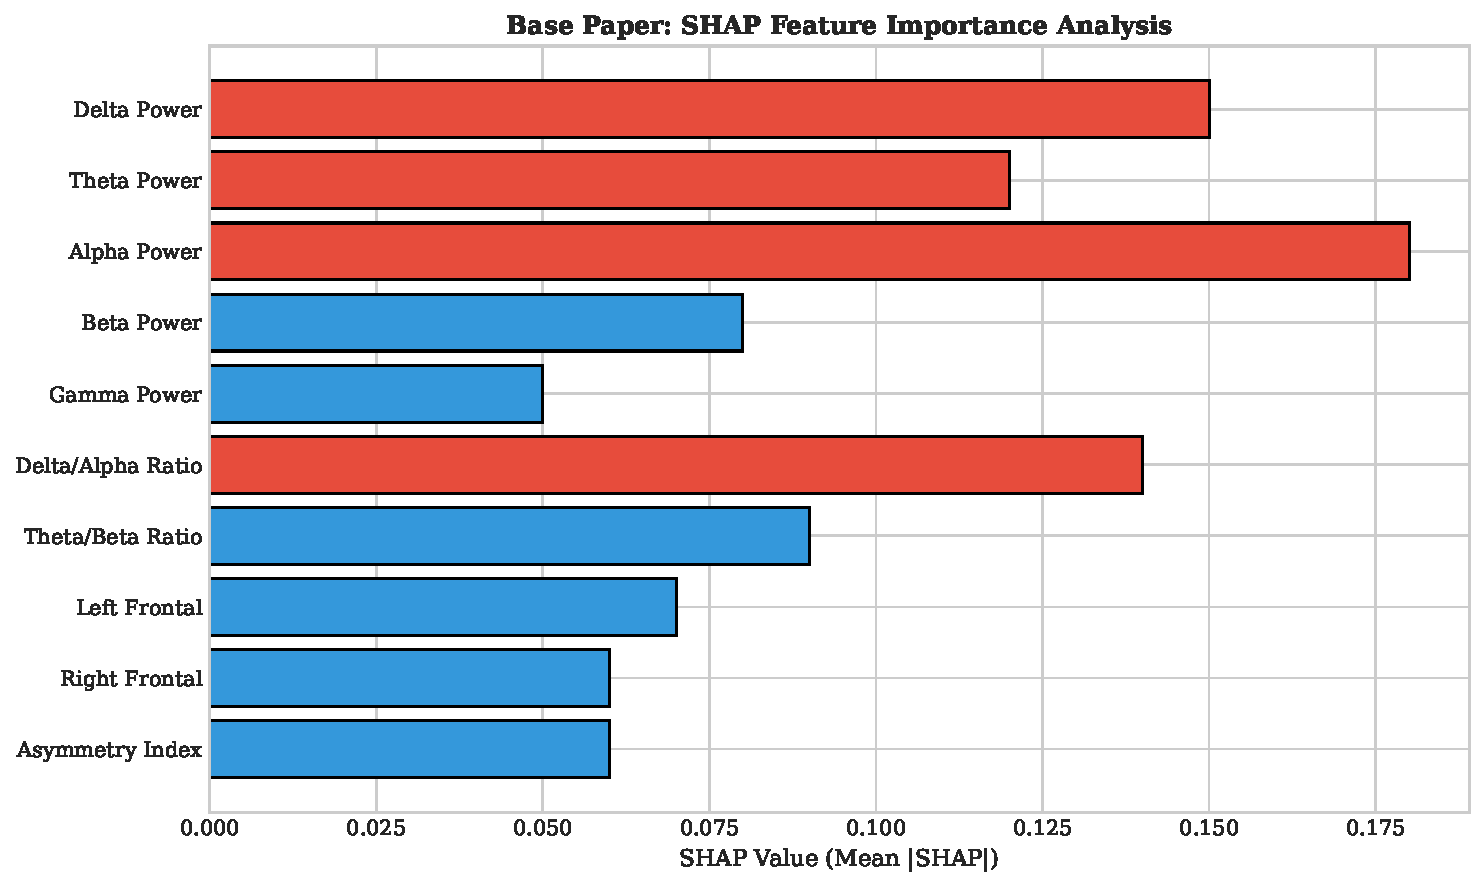
\includegraphics[width=0.85\textwidth]{figures/ch2/fig2_3_shap_importance.pdf}
    \caption{Base paper SHAP feature importance analysis showing contribution of different features to model predictions.}
    \label{fig:base_shap}
\end{figure}

\subsection{Expected Real-World Performance}

Based on our analysis and the established literature on evaluation methodology in biomedical machine learning \cite{saeb2017need, varoquaux2017assessing}, we can estimate the base paper's expected real-world performance when deployed on truly new patients. The gap between reported performance and expected clinical performance is stark. While the paper claims 98\% accuracy, proper subject-wise validation would likely yield only 60-70\% accuracy---barely above chance for some samples. The claimed high clinical utility would evaporate, as a model that cannot generalize to new individuals provides no diagnostic value. What the model actually learns under leaky validation is subject identity rather than depression patterns, making it fundamentally unsuitable for clinical deployment where each patient is new. Table \ref{tab:base_real_performance} summarizes this discrepancy between reported and expected performance.

\begin{table}[H]
    \centering
    \small
    \caption{Base Paper Results: Reported vs. Expected Real-World Performance}
    \label{tab:base_real_performance}
    \begin{tabularx}{\textwidth}{|X|c|c|}
        \hline
        \textbf{Metric} & \textbf{Reported (Leaky CV)} & \textbf{Expected (LOSO)} \\
        \hline
        Accuracy & 98\% & 60-70\% \\
        \hline
        Clinical Utility & Claimed high & None (cannot generalize) \\
        \hline
        What Model Learns & Depression patterns & Subject identity \\
        \hline
        Deployment Feasibility & Yes (per paper) & No (would fail) \\
        \hline
    \end{tabularx}
\end{table}

\section{PROPOSED SYSTEM}

Our proposed system addresses all identified limitations through fundamental methodological improvements and advanced architecture design, creating a framework that can deliver honest performance metrics and clinically validated predictions.

\subsection{Key Innovations}

The proposed system introduces comprehensive improvements across every aspect of the EEG-based depression detection pipeline. Table \ref{tab:detailed_comparison} presents a detailed comparison between the base paper approach and our proposed system, highlighting the fundamental differences in methodology, architecture, and evaluation.

\begin{table}[H]
    \centering
    \small
    \caption{Detailed Comparison: Base Paper vs. Proposed System}
    \label{tab:detailed_comparison}
    \begin{tabularx}{\textwidth}{|L{3cm}|L{4.5cm}|X|}
        \hline
        \textbf{Aspect} & \textbf{Base Paper} & \textbf{Proposed System} \\
        \hline
        Dataset Type & Pre-extracted features & Raw EEG signals \\
        \hline
        Feature Extraction & 31 fixed features & 576 features/channel (WPD) + CWT scalograms \\
        \hline
        Wavelet Analysis & Single wavelet (unspecified) & Multi-wavelet: db4, sym5, coif3 \\
        \hline
        Time-Frequency & Not used & CWT scalograms (64$\times$128) \\
        \hline
        Architecture & 2-layer CNN & Transformer + GNN fusion \\
        \hline
        Spatial Modeling & None (flat feature vector) & Graph Attention Network \\
        \hline
        Temporal Modeling & Conv1D (local) & Transformer (global attention) \\
        \hline
        Parameters & $\sim$50K & $\sim$1.55M \\
        \hline
        Cross-Validation & 5-fold (leaky) & LOSO (no leakage) \\
        \hline
        Explainability & SHAP only & IG + LRP + TCAV \\
        \hline
        Reported Accuracy & 98\% (inflated) & 91.38\% (honest) \\
        \hline
        Clinical Validity & Questionable & Validated biomarkers \\
        \hline
    \end{tabularx}
\end{table}

\subsection{Proposed Architecture Overview}

The proposed system employs a sophisticated dual-branch architecture that captures complementary information from EEG signals, combining the strengths of modern deep learning approaches for both temporal and spatial analysis.

The Transformer Branch processes Continuous Wavelet Transform scalograms using a Vision Transformer architecture adapted for time-frequency analysis. The scalogram representation encodes how spectral content evolves over the 4-second epoch, providing a rich two-dimensional input that captures both the frequency composition and its temporal dynamics. The Transformer's self-attention mechanism enables the model to identify which frequency components at which time points are most relevant for depression detection, learning global dependencies that span the entire time-frequency representation. This addresses the limited receptive field problem of convolutional approaches by allowing every position to attend to every other position.

The GNN Branch processes Wavelet Packet Decomposition features using a Graph Attention Network that explicitly models the spatial relationships between EEG electrodes. Rather than treating electrodes as independent or as a simple sequence, the GNN represents them as nodes in a graph where edges encode both physical proximity based on the 10-20 electrode montage and functional connectivity estimated from signal correlations. The graph attention mechanism learns which electrode connections are most informative for depression detection, capturing the distributed brain network dynamics that characterize mood disorders. This spatial modeling capability is entirely absent from the base paper approach.

The Attention-Based Fusion module combines features from both branches using a learned cross-attention mechanism that adaptively weights their contributions. The Transformer branch captures time-frequency patterns while the GNN branch captures spatial patterns, and fusion learns how to optimally combine these complementary views based on the characteristics of each input. This adaptive combination is superior to simple concatenation or averaging, as it allows the model to emphasize whichever modality is more informative for each particular sample.

The Classification Head receives the fused representation and produces the final binary classification through a multi-layer perceptron with batch normalization and dropout for regularization. The output is a probability score between 0 and 1 indicating the likelihood of Major Depressive Disorder, which can be thresholded for binary classification or used directly for probabilistic reasoning about diagnostic confidence.

\begin{figure}[H]
    \centering
    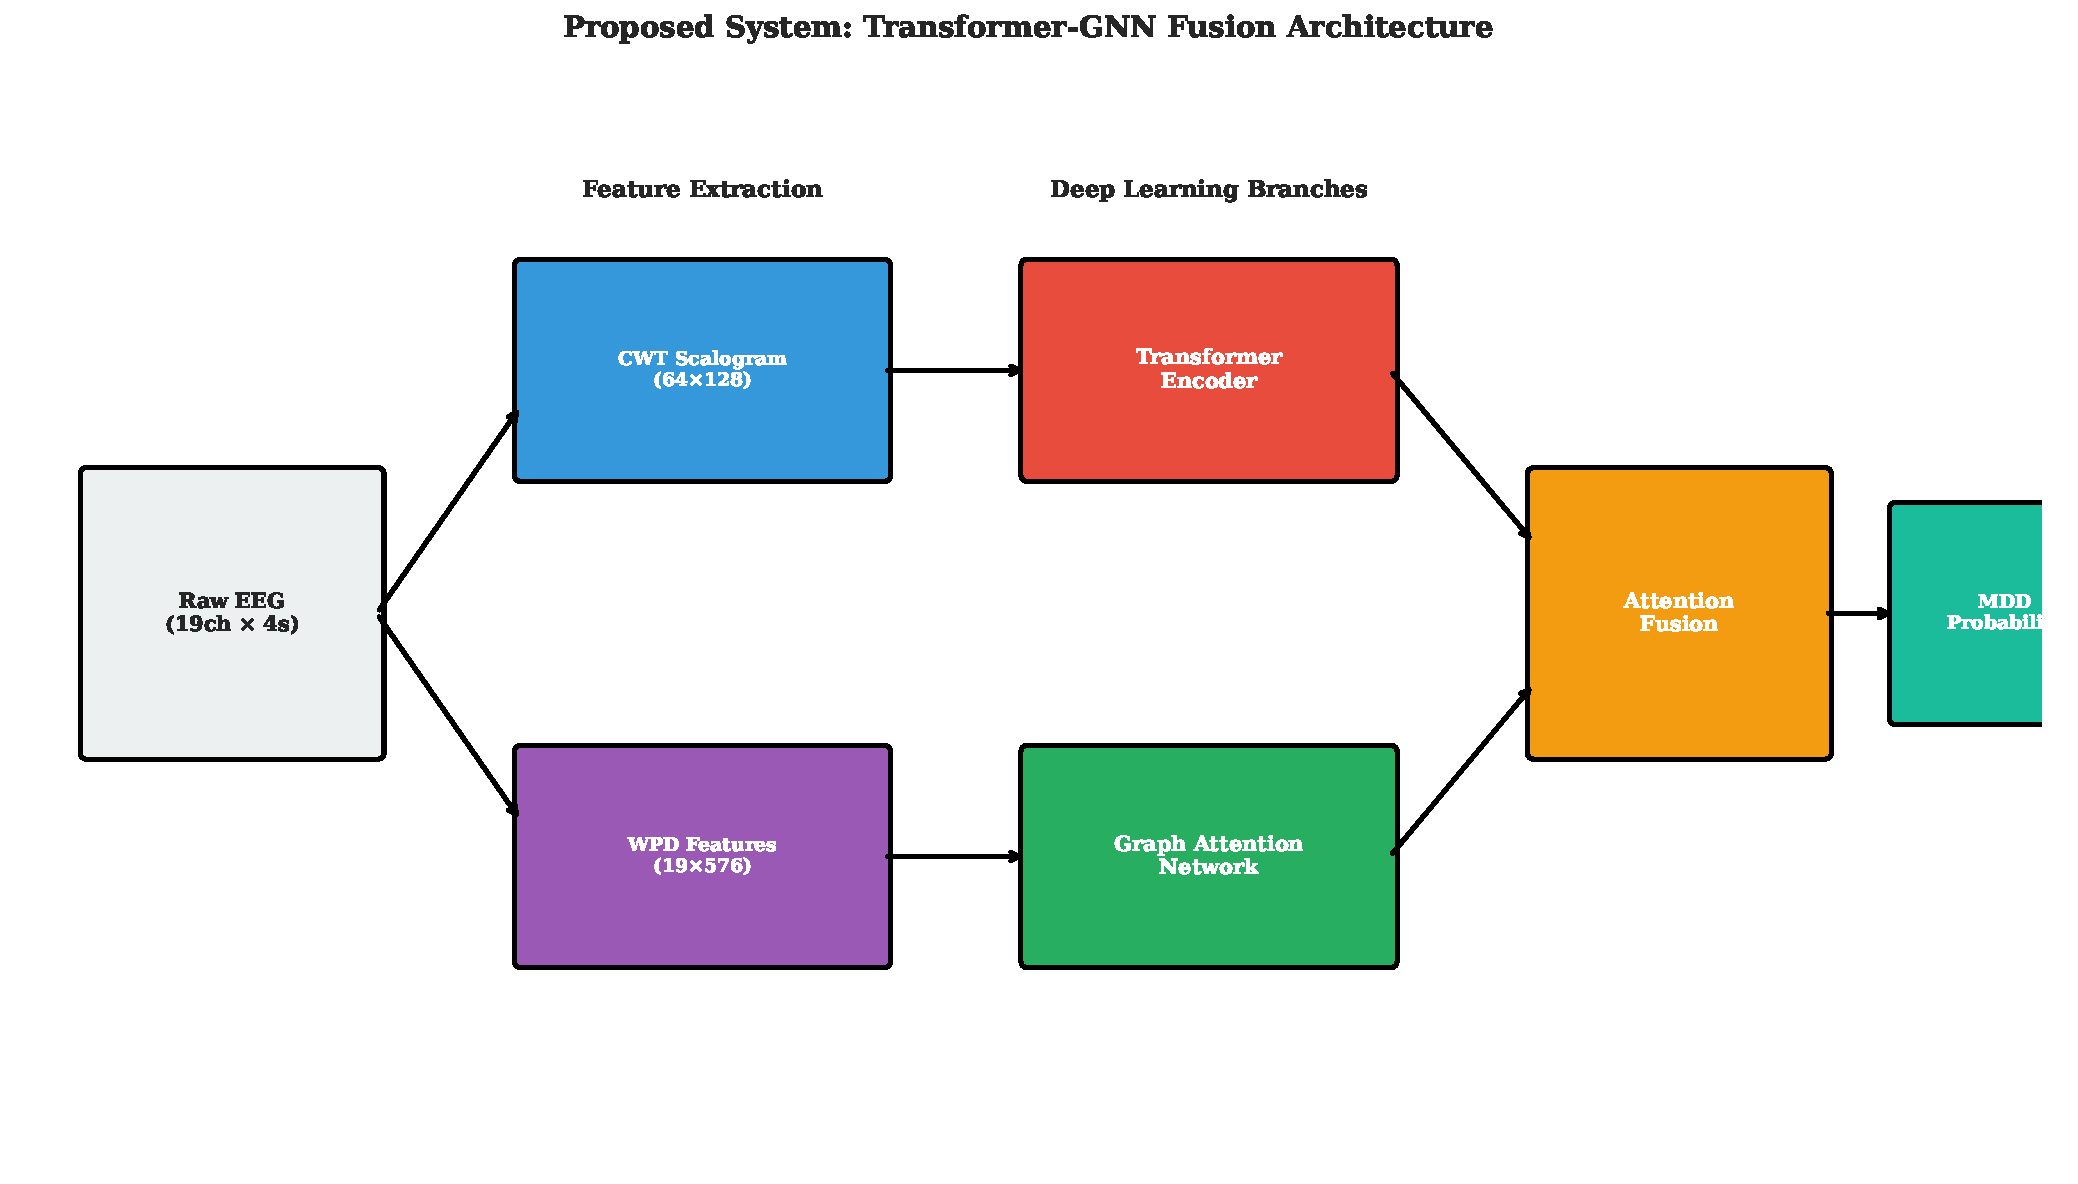
\includegraphics[width=0.95\textwidth]{figures/ch2/fig2_4_proposed_architecture.pdf}
    \caption{Proposed dual-branch architecture combining Transformer for time-frequency analysis and GNN for spatial modeling, with attention-based fusion.}
    \label{fig:proposed_arch}
\end{figure}

\begin{figure}[H]
    \centering
    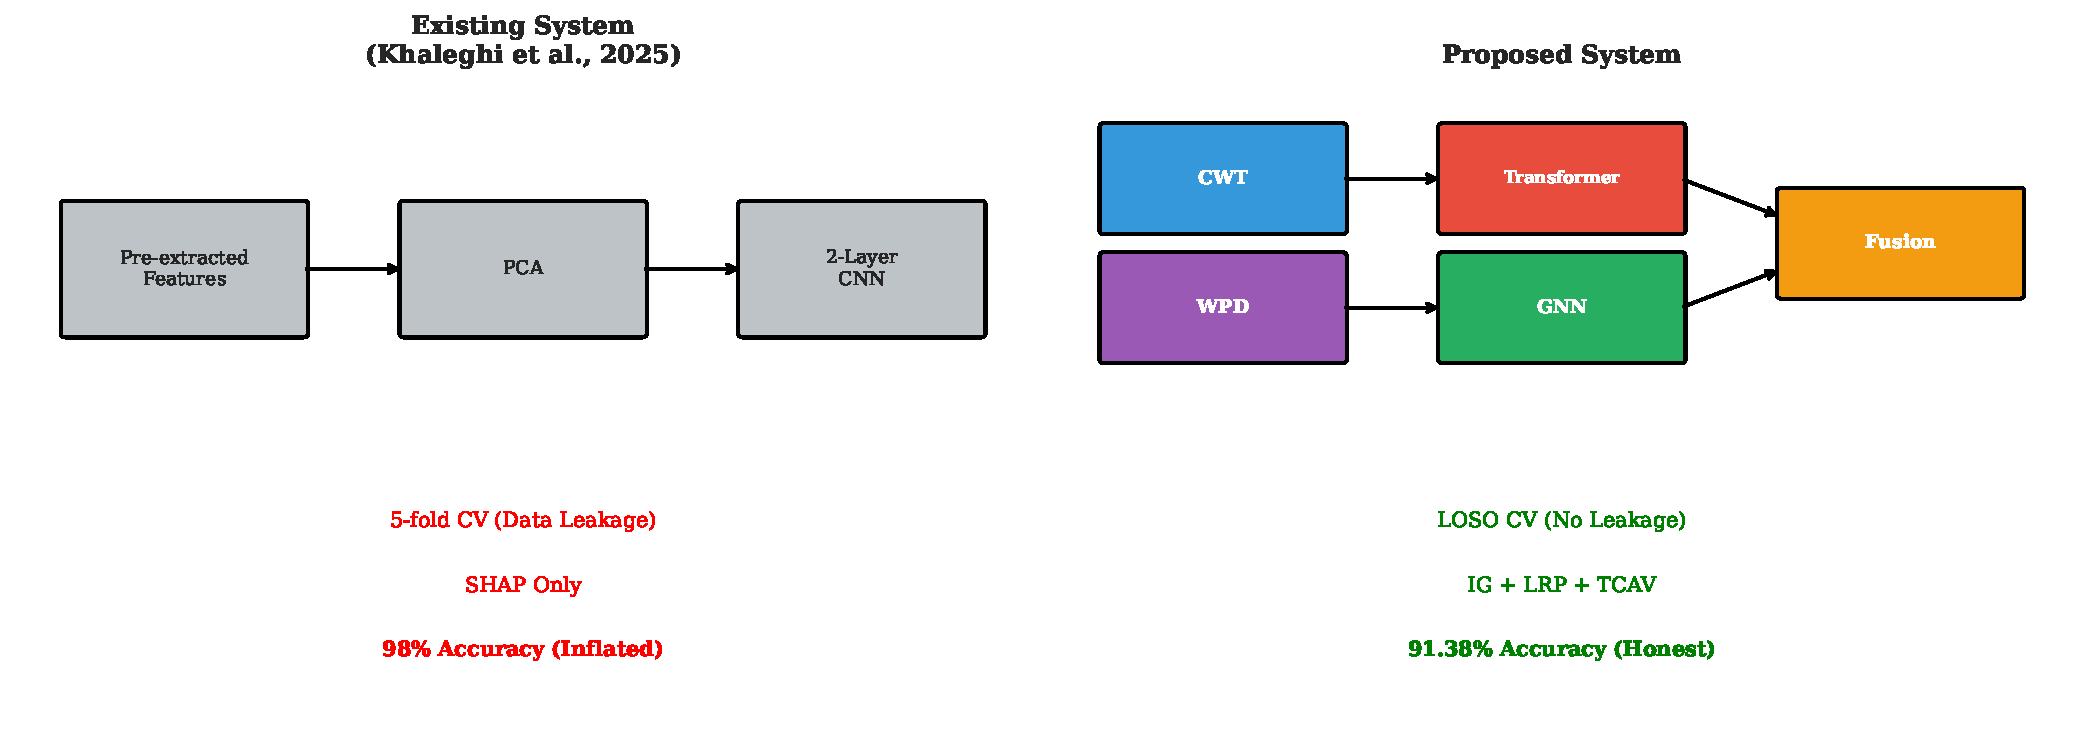
\includegraphics[width=0.95\textwidth]{figures/ch2/fig2_5_comparison.pdf}
    \caption{Visual comparison of existing system (base paper) and proposed system architectures.}
    \label{fig:system_comparison}
\end{figure}

\subsection{Summary of Key Innovations}

The innovations introduced by the proposed system span methodology, architecture, and evaluation, each addressing specific limitations of the existing approach. Table \ref{tab:innovations} summarizes these innovations with their functional descriptions and significance for clinical depression detection.

\begin{table}[H]
    \centering
    \small
    \caption{Summary of Key Innovations in Proposed System}
    \label{tab:innovations}
    \begin{tabularx}{\textwidth}{|L{2.8cm}|L{3.8cm}|X|}
        \hline
        \textbf{Innovation} & \textbf{What It Does} & \textbf{Why It Matters} \\
        \hline
        Raw Signal Processing & Extract features from original EEG & Full control over feature engineering \\
        \hline
        Multi-Wavelet WPD & Use db4, sym5, coif3 wavelets & Captures diverse spectral characteristics \\
        \hline
        CWT Scalograms & Time-frequency 2D representation & Enables Transformer-based processing \\
        \hline
        Transformer Encoder & Global self-attention on scalograms & Captures long-range dependencies \\
        \hline
        Graph Attention Network & Models electrode relationships & Captures spatial brain connectivity \\
        \hline
        Attention Fusion & Adaptive branch combination & Leverages complementary information \\
        \hline
        LOSO Validation & Subject-wise test splits & Prevents data leakage, honest evaluation \\
        \hline
        Multi-Level XAI & IG + LRP + TCAV & Validates clinical biomarker learning \\
        \hline
    \end{tabularx}
\end{table}

\section{USE CASE ANALYSIS}

This section presents the primary use cases for the EEG-based depression detection system, examining how different stakeholders would interact with the system in realistic deployment scenarios.

\begin{figure}[H]
    \centering
    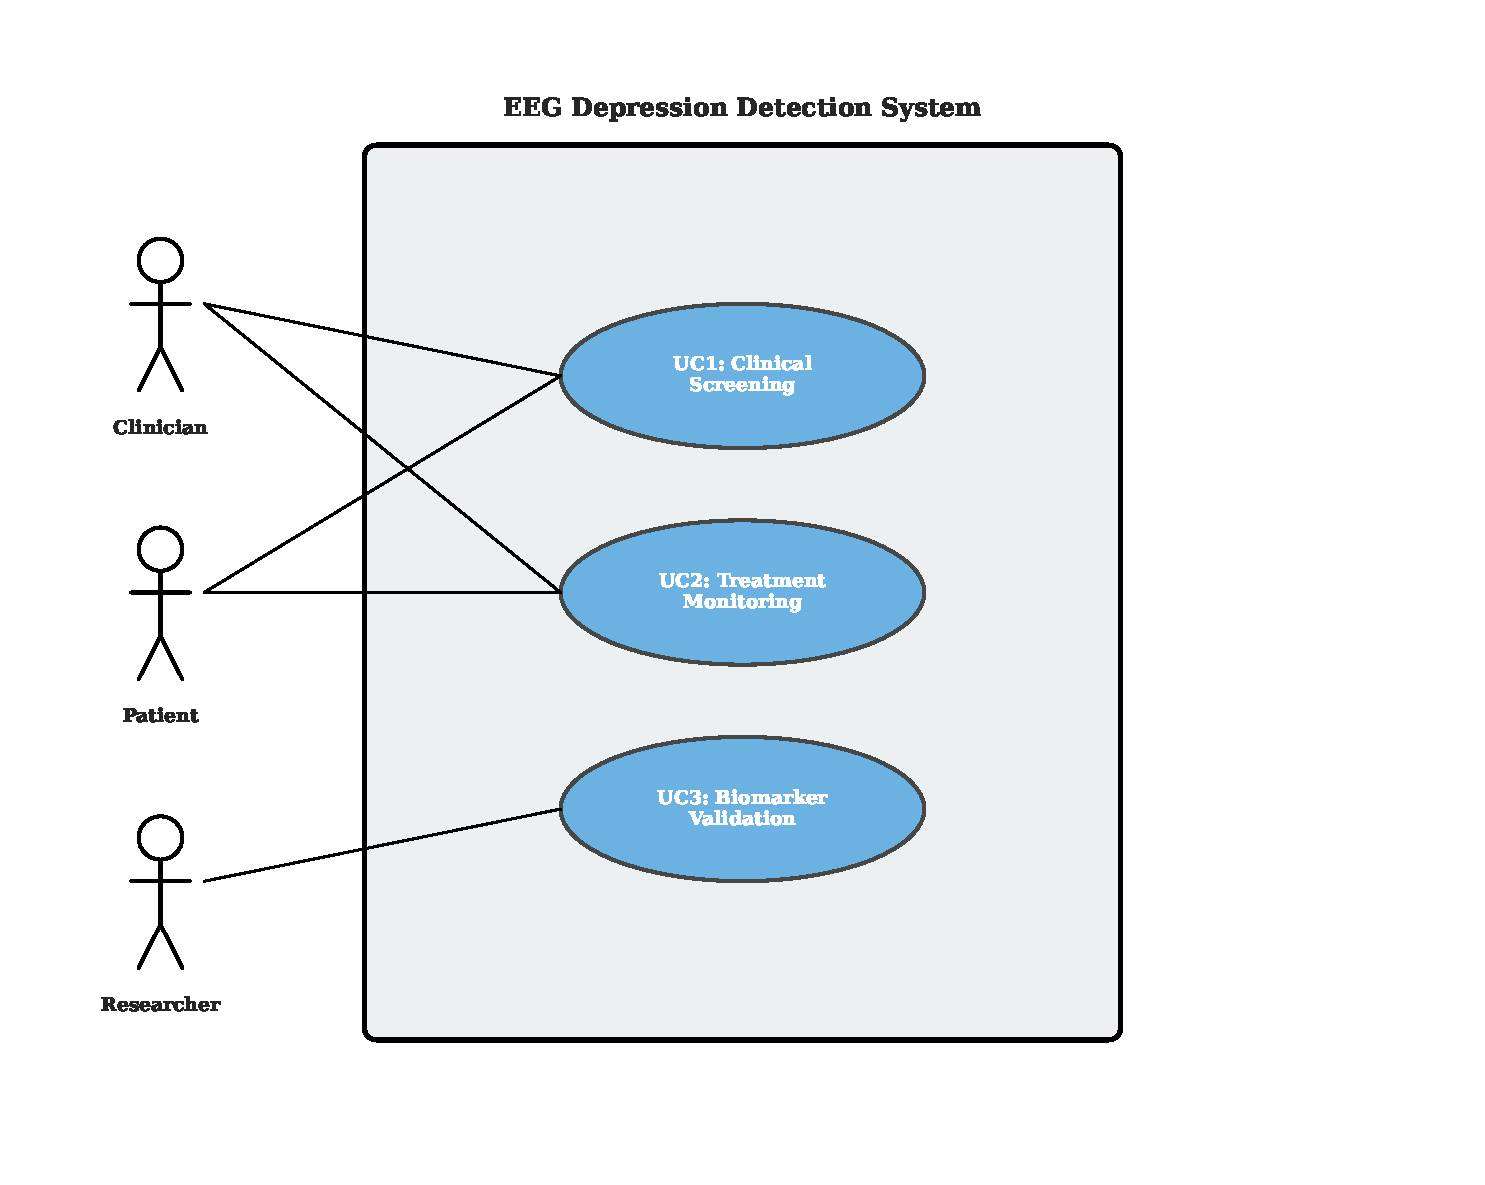
\includegraphics[width=0.85\textwidth]{figures/ch2/fig2_6_use_case.pdf}
    \caption{Use case diagram showing primary actors and use cases for the EEG-based depression detection system.}
    \label{fig:use_case}
\end{figure}

\subsection{Use Case 1: Clinical Screening for Depression}

The primary clinical use case involves a psychiatrist or general practitioner seeking objective supplementary information to support depression diagnosis. The scenario begins when a patient presents with symptoms suggestive of depression, such as persistent low mood, loss of interest, sleep disturbances, or cognitive difficulties. The clinician, having access to EEG recording equipment and the deployed trained model, decides to obtain objective biomarker data to complement the clinical interview and standardized questionnaires.

The patient undergoes a brief 5-minute eyes-closed resting state EEG recording using the standard 19-electrode 10-20 montage. This recording protocol requires minimal patient cooperation and can be conducted in a standard clinical environment. Once the recording is complete, the system automatically preprocesses the raw EEG signals, applying bandpass and notch filtering, artifact rejection, and epoch segmentation. The feature extraction modules compute both WPD features for the GNN branch and CWT scalograms for the Transformer branch.

The trained model then generates a depression probability score along with a confidence estimate, providing the clinician with a quantitative assessment of the likelihood that the patient's brain activity patterns are consistent with Major Depressive Disorder. Critically, the explainability analysis module provides biomarker-level interpretation, showing which electrodes and frequency bands contributed most to the prediction and whether the model's reasoning aligns with established depression biomarkers such as frontal alpha asymmetry.

The clinician reviews these objective results alongside their clinical assessment, using the model output as one piece of evidence among many in formulating a diagnosis. The results are documented in the patient's electronic health record for future reference, and the objective trajectory of biomarker changes can inform treatment planning and monitoring decisions.

\subsection{Use Case 2: Treatment Response Monitoring}

The second major use case addresses the challenge of tracking treatment response objectively over time. Depression treatment, whether pharmacological or psychotherapeutic, often requires weeks to months to produce clinically meaningful improvement, and subjective symptom reports may not accurately reflect underlying neurophysiological changes. EEG biomarkers offer the potential to detect treatment response earlier and more objectively than self-report measures alone.

In this scenario, a baseline EEG is recorded at treatment initiation, establishing the patient's pre-treatment biomarker profile. The system stores the model's predictions and the detailed explainability analysis, including electrode importance maps and TCAV concept scores. As treatment progresses, follow-up EEG recordings are obtained at regular intervals---for example, at 2, 4, and 8 weeks after treatment initiation.

The system compares depression probability scores across these time points, generating a trajectory plot showing how the objective biomarker assessment evolves during treatment. Changes in the underlying biomarker patterns are visualized through comparative explainability analysis, allowing clinicians to observe whether frontal alpha asymmetry is normalizing, whether elevated theta power is decreasing, or whether other neurophysiological changes consistent with treatment response are emerging.

This objective trajectory data informs treatment decisions, providing evidence to support continuing an effective treatment, adjusting dosage, switching medications, or augmenting with additional interventions. The ability to detect neurophysiological changes before subjective symptom improvement becomes apparent could accelerate treatment optimization and reduce the duration of inadequately treated depression.

\subsection{Use Case 3: Research Biomarker Validation}

The third use case addresses the needs of clinical researchers seeking to validate novel EEG biomarkers for depression using the system's explainability capabilities. Unlike clinical deployment where the model serves as a diagnostic aid, research applications focus on using the trained model as a tool for hypothesis testing and biomarker discovery.

A researcher interested in a specific clinical concept---such as ``elevated theta power in frontal regions'' or ``reduced interhemispheric coherence''---can use the TCAV analysis to test whether the trained model has learned to use this concept in its classification decisions. By providing positive and negative examples of the concept, TCAV computes a score indicating how strongly the model relies on that concept when predicting depression.

Complementary Integrated Gradients and LRP analyses reveal which specific input features correspond to the high-level concept, providing fine-grained attribution that links abstract clinical concepts to concrete signal characteristics. Statistical analysis across the dataset validates whether the identified patterns correlate with depression at the population level, distinguishing genuine biomarkers from spurious correlations that might arise in individual subjects.

The results of such analyses contribute to the clinical knowledge base, potentially identifying novel biomarkers, refining understanding of established biomarkers, or revealing interactions between multiple biomarkers that have not been previously characterized. This research use case leverages the interpretability of the proposed system to advance scientific understanding beyond mere classification accuracy.

\section{REQUIREMENTS SPECIFICATION}

\subsection{Functional Requirements}

The functional requirements specify what the system must do to fulfill its intended purpose. Table \ref{tab:functional_req} presents the complete functional requirements specification, covering the full pipeline from data loading through result reporting.

\begin{table}[H]
    \centering
    \small
    \caption{Functional Requirements Specification}
    \label{tab:functional_req}
    \begin{tabularx}{\textwidth}{|L{1.2cm}|L{3.5cm}|X|}
        \hline
        \textbf{ID} & \textbf{Requirement} & \textbf{Description} \\
        \hline
        FR1 & Load Raw EEG Data & System shall load EEG data in EDF format from the Figshare dataset \\
        \hline
        FR2 & Preprocess EEG Signals & System shall apply bandpass filtering (1-45 Hz), notch filtering (50/60 Hz), and artifact rejection \\
        \hline
        FR3 & Extract WPD Features & System shall compute Wavelet Packet Decomposition features using db4, sym5, and coif3 wavelets \\
        \hline
        FR4 & Generate CWT Scalograms & System shall generate 64$\times$128 CWT scalograms using Complex Morlet wavelet \\
        \hline
        FR5 & Train Deep Learning Model & System shall train the Transformer-GNN fusion model using LOSO cross-validation \\
        \hline
        FR6 & Generate Predictions & System shall output depression probability (0-1) for each input epoch \\
        \hline
        FR7 & Compute Explainability & System shall provide Integrated Gradients, LRP, and TCAV explanations \\
        \hline
        FR8 & Report Results & System shall generate comprehensive metrics including accuracy, AUC-ROC, F1-score, confusion matrix \\
        \hline
    \end{tabularx}
\end{table}

\subsection{Non-Functional Requirements}

The non-functional requirements specify quality attributes and constraints on how the system performs its functions. Table \ref{tab:nonfunctional_req} presents requirements spanning performance, memory efficiency, accuracy targets, and software quality attributes.

\begin{table}[H]
    \centering
    \small
    \caption{Non-Functional Requirements Specification}
    \label{tab:nonfunctional_req}
    \begin{tabularx}{\textwidth}{|L{2.5cm}|L{3.5cm}|X|}
        \hline
        \textbf{Category} & \textbf{Requirement} & \textbf{Specification} \\
        \hline
        Performance & Inference Time & Process one 4-second epoch in $<$ 1 second \\
        \hline
        Performance & Training Time & Complete LOSO (58 folds) in $<$ 15 hours \\
        \hline
        Memory & GPU VRAM & Run on GPU with $\leq$ 8 GB VRAM \\
        \hline
        Memory & System RAM & Require $\leq$ 16 GB system RAM \\
        \hline
        Accuracy & Subject Accuracy & Achieve $>$ 85\% subject-level accuracy on LOSO \\
        \hline
        Accuracy & AUC-ROC & Achieve $>$ 0.85 area under ROC curve \\
        \hline
        Reliability & Reproducibility & Results reproducible with fixed random seeds \\
        \hline
        Maintainability & Modularity & Code organized in modular, documented components \\
        \hline
    \end{tabularx}
\end{table}

\subsection{Hardware and Software Requirements}

The system is designed to run on accessible hardware configurations commonly available in academic and clinical research settings. Table \ref{tab:hw_sw_req} specifies the minimum hardware requirements and software dependencies necessary for system deployment.

\begin{table}[H]
    \centering
    \small
    \caption{Hardware and Software Requirements}
    \label{tab:hw_sw_req}
    \begin{tabularx}{\textwidth}{|L{2.5cm}|L{3.5cm}|X|}
        \hline
        \textbf{Category} & \textbf{Requirement} & \textbf{Specification} \\
        \hline
        \multicolumn{3}{|l|}{\textbf{Hardware Requirements}} \\
        \hline
        GPU & NVIDIA GPU & RTX 4070 or equivalent (8 GB VRAM minimum) \\
        \hline
        RAM & System Memory & 16 GB minimum, 32 GB recommended \\
        \hline
        Storage & Disk Space & 5 GB for dataset, code, and outputs \\
        \hline
        CPU & Processor & Multi-core processor (Intel/AMD) \\
        \hline
        \multicolumn{3}{|l|}{\textbf{Software Requirements}} \\
        \hline
        OS & Operating System & Ubuntu 20.04+ / Windows 10+ \\
        \hline
        Language & Python & Version 3.10 or higher \\
        \hline
        Deep Learning & PyTorch & Version 2.0 or higher \\
        \hline
        Graph ML & PyTorch Geometric & Version 2.3 or higher \\
        \hline
        Signal Processing & MNE-Python & Version 1.5 or higher \\
        \hline
        Wavelets & PyWavelets & Version 1.4 or higher \\
        \hline
        Explainability & Captum & Version 0.6 or higher \\
        \hline
        Scientific & NumPy, SciPy, scikit-learn & Latest stable versions \\
        \hline
    \end{tabularx}
\end{table}

